\chapter{Harmonogram prac}
\section{Diagram Gantta}

Diagram Gantta to narzędzie wykorzystywane do przedstawiania harmonogramu zadań w czasie. Składa się z osi poziomej reprezentującej czas oraz osi pionowej przedstawiającej zadania. Każde zadanie jest przedstawiane za pomocą prostokąta, a jego długość odpowiada czasowi trwania zadania.\newline

Na diagramie Gantta reprezentującym harmonogram pracy podczas tworzenia aplikacji sklepu znajduje się również legenda, która opisuje kolory użyte do prezentacji zadania. Kolor pomarańczowy reprezentuje prace projektowe oraz analityczne. Zazwyczaj takie prace wykonywane są jako pierwsze jeszcze przed implementacją kodu. Na podstawie ustaleń w tym procesie powstaje architektura projektu.\newline

Kolorem niebieskim oznaczono prace frontowe odpowiadajace za wygląd aplikacji. Najczęściej prace te wykonywane są jednocześnie z pracami backendowymi. Jednak w przypadku aplikacji konsolowej najpierw wykonano prace odpowiadające za wizualną formę programu.\newline

Kolorem zielonym zaznaczono na diagramie prace nad implementacją operacji i mechanizmów logicznych.\newline

\begin{figure}[!ht]
	\centering
		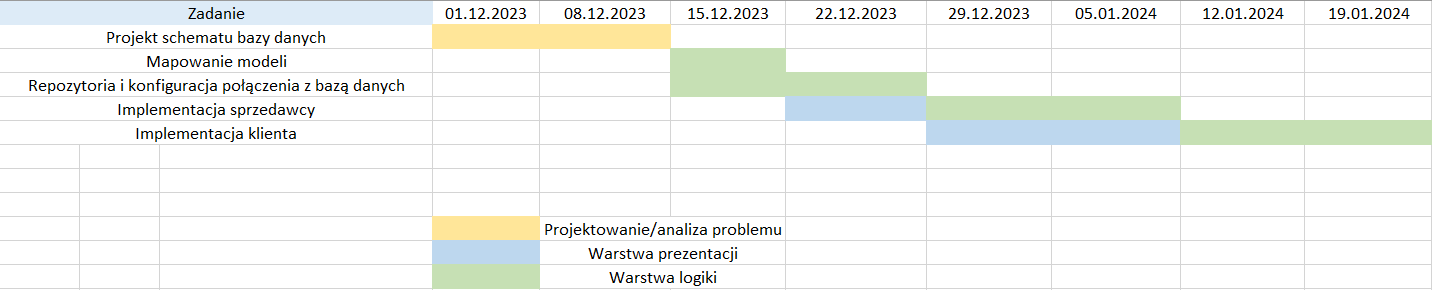
\includegraphics[width=15cm]{gant.png}
	\caption{\footnotesize Diagram Gantta}
	\label{fig:plotend}
\end{figure}